\pdfoutput=1
% ^ arXiv detects a pdflatex submission from this line; keep it within
%   the first five lines of the file.
\documentclass[10pt]{article}

\usepackage[biblatex]{flockpaper}

\usepackage{subcaption}
\usepackage{nicefrac}
\usepackage{algorithm2e}

\usepackage[backend=biber]{biblatex}
\addbibresource{refs.bib}
\renewcommand*{\bibfont}{\normalfont\small}

% allow long URLs in the bibliography to break across lines
\setcounter{biburlnumpenalty}{9000}
\setcounter{biburlucpenalty}{9000}
\setcounter{biburllcpenalty}{9000}

\usetikzlibrary{arrows.meta, bending, positioning}

\newcommand{\map}{\mathop{\bigoplus}\limits}
\newcommand{\txtop}[1]{\mathop{\mathtt{#1}}\limits}

% a table header cell on two lines: \stackhead[r]{loss\\recovered}
\newcommand{\stackhead}[2][l]{\begin{tabular}[b]{@{}#1@{}}#2\end{tabular}}

\newcommand{\expr}{\txtop{expression}}

\newcommand{\fn}{\txtop{function}}
\newcommand{\linear}{\txtop{linear}}
\newcommand{\relu}{\txtop{ReLU}}
\newcommand{\topk}{\txtop{TopK}}
\newcommand{\sigmoid}{\txtop{sigmoid}}
\newcommand{\tanhl}{\txtop{tanh}}
\newcommand{\softmax}{\txtop{softmax}}
\newcommand{\argmin}{\txtop{argmin}}
\newcommand{\argmax}{\txtop{argmax}}
\newcommand{\einsum}{\txtop{einsum}}
\newcommand{\colsum}{\txtop{colsum}}

\newcommand{\encoder}{\txtop{encoder}}
\newcommand{\decoder}{\txtop{decoder}}
\newcommand{\classifier}{\txtop{classifier}}
\newcommand{\partitioner}{\txtop{dict}}

\newcommand{\bilinear}{\txtop{Bilinear}}
\newcommand{\bilinearblock}{\txtop{BilinearBlock}}
\newcommand{\dictblock}{\txtop{DictBlock}}
\newcommand{\dictenc}{\txtop{DictEnc}}
\newcommand{\ontologizer}{\txtop{Ontologizer}}

\SetKwProg{Fn}{Function}{}{end}
\SetKwProg{Dat}{Data}{}{end}

\SetKwInOut{Hyper}{Hyperparameters}

\SetKwFunction{softmax}{softmax}
\SetKwFunction{MSE}{MSE}
\SetKwFunction{L1}{L1}
\SetKwFunction{transpose}{transpose}
\SetKwFunction{matmul}{matmul}
\SetKwFunction{dist}{dist}
\SetKwFunction{eucl}{euclidean}
\SetKwFunction{cossim}{cossim}
\SetKwFunction{sindiff}{sindiff}
\SetKwFunction{pca}{pca}
\SetKwFunction{knn}{knn}

\SetKwFunction{sample}{sample}
\SetKwFunction{loss}{loss}
\SetKwFunction{train}{train}

\SetKwFunction{Type}{Type}
\SetKwFunction{List}{List}
\SetKwFunction{Arch}{Arch}
\SetKwFunction{Params}{Params}
\SetKwFunction{Model}{Model}

\SetKwFunction{Linear}{Linear}
\SetKwFunction{Bilinear}{Bilinear}
\SetKwFunction{NLinear}{NLinear}
\SetKwFunction{NLinearBlock}{NLinearBlock}
\SetKwFunction{DictBlock}{DictBlock}
\SetKwFunction{DictEnc}{DictEnc}
\SetKwFunction{Ontologizer}{Ontologizer}
\SetKwFunction{SAE}{SAE}


\title{A proposal for interpreting dense networks}
\author{%
  \begin{tabular}[t]{@{}l@{\hspace{2em}}l@{}}
    Keira Wiechecki & Lamb Wakefield \\[2pt]
    \mutedlabel{Wakaru \textperiodcentered{} kaw504@nyu.edu} &
    \mutedlabel{Flock Capital \textperiodcentered{} lamb@flock.holdings} \\[6pt]
    Jade Zaslavsky & vmfunc \\[2pt]
    \mutedlabel{Wakaru \textperiodcentered{} jadeofnameless@gmail} &
    \mutedlabel{Flock Capital \textperiodcentered{} celeste@linux.com}
  \end{tabular}}
\date{\today}
\eyebrow{proposal \textperiodcentered{} preliminary results \textperiodcentered{} mechanistic interpretability}
\runningtitle{Dictionary learning is all you need}
\begin{document}
\maketitle

% Frontispiece: decorative, deliberately not a numbered float.
\noindent\plate{
\includegraphics[width=\dimexpr\textwidth-0.8pt\relax]{figures/frontis-orbit.png}}\\[3pt]
\mutedlabel{orbit \textperiodcentered{} seed 1024 \textperiodcentered{} floyd\textendash{}steinberg error diffusion}
\vspace{16pt}

\begin{abstract}
% flockpaper sets the abstract in an unbreakable minipage, so it must fit
% on the page it starts on or it moves to the next one whole
\small
Behavioral evaluation cannot settle what a model is trying to do, since a
model can behave differently when it believes it is being trained or
evaluated. Settling it means identifying the model's variables, including
ones no one has named: the ontology identification problem. Supervised
probes and difference-of-means vectors now beat sparse autoencoder (SAE)
features at detection and steering, but supervision only confirms concepts
someone already suspects. We argue that unsupervised methods lose partly
because of what they return: an SAE latent fires or stays silent, and
absorption makes its silence uninformative, while the methods that win
contrast the values of a variable. We propose learning variables
directly, as competitive classifier heads that give every input one of $k$
entries whose atoms reconstruct it. Forcing a head to another entry is
then a label-free difference of means, and steering can test a
discovered variable, though only against arbitrary partitions of the
same space, a baseline not yet run here. Preliminary results on SONAR sentence
embeddings and GPT-2 residuals: trained heads are contrast sets; a pure
1900-bit hard code reconstructs at least 33\% better than a $\topk$ SAE
held to the same bits, though an entropy-coded L1 SAE does better still;
on GPT-2 an 800-bit code recovers more of the model's loss than a
$k_{\mathrm{SAE}}{=}32$ SAE; in the soft code, forced entries steer along
the supervised difference-of-means direction $0.64\times$ as far as
supervised steering and $4\times$ as far as probe directions; and
interventions set on heads compose nearly additively. But the variables are not yet
identifiable: seeds agree on the error to four digits but share no head
past the first layer, input-space steps disturb other heads as much as
random steps of the same length, and weight-only decodes do not describe
entries. Identifiability, not fidelity, is the binding constraint, for
auditing and for any goal that must keep pointing at one concept as a
model is retrained, and it is where the proposed work begins.
\end{abstract}

\section{Introduction}

Ideally we would like mechanistic interpretability to provide guarantees
about the computational process used by a model. We would like features
to be
\begin{enumerate}
	\item causal
	\item disentangled
	\item closed-form
\end{enumerate}
However most existing techniques, such as sparse autoencoders (SAEs),
produce features that can perform arbitrarily badly on these desiderata.
As a dictionary grows, features split into narrower
ones~\cite{bricken2023}, and a narrow feature can absorb a broader one,
which then fails to fire where it applies~\cite{chanin2025}, so the code
is not disentangled. SAE features can't usually be
statically analyzed (though bilinear SAE variants can be). Sparsity
trades off against reconstruction fidelity, limiting the extent to which
features can be used for steering.

Arguably the simplest interpretability technique is a linear probe, and
the simplest control technique is a steering vector. On current
benchmarks both beat features from unsupervised techniques such as SAEs,
probes at detecting concepts and the difference of means at steering
them~\cite{wu2025axbenchsteeringllmssimple}, but they require contrastive
data built around a concept someone has already named, labeled or
not~\cite{burns2023ccs}. In the spirit of MoEfication~\cite{zhang2022}, we
propose a technique based on decomposing a representation space into a
set of contrastive classifiers. Each class corresponds to a representative vector. Inputs
are encoded as a series of classifications, and reconstructed from the
representative vectors those classifications select. This has several
advantages over SAEs:
\begin{enumerate}
	\item It effectively gives steering for free: changing a
	classification is a steering move.
	\item Outputs are bounded.
	\item The representative vectors admit static interpretation in
	principle; making that real is currently an open problem
	(Section~\ref{sec:prelim-autointerp}).
	\item Feature space is structured.
\end{enumerate}
The steering primitive, measured, is Figure~\ref{fig:teaser}; the
evaluation so far, including where it cuts against the proposal, is
Section~\ref{sec:prelim}.

\begin{figure}[tp]\centering
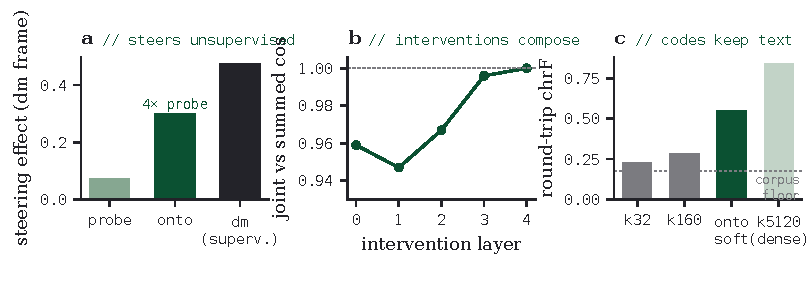
\includegraphics[width=\linewidth]{figures/fig-teaser.pdf}
\caption[The steering primitive, measured]{The softmax Ontologizer's
steering primitive, measured. (a) Forcing an entry moves decodes along
the supervised difference-of-means direction $0.64\times$ as far as
supervised steering itself and $4\times$ as far as probe directions
(Table~\ref{tab:steer-overlay}). (b) Joint two-head interventions
point where the summed single interventions point, exactly in the final
layer. (c) The sparse SAEs' codes lose most text before any
intervention (round-trip chrF 0.23--0.28 against a 0.18 corpus floor)
while the soft code keeps it (0.55); the dense $k_{\mathrm{SAE}}{=}5120$ SAE keeps more
but is not a sparse code.}
\label{fig:teaser}
\end{figure}

\section{Assumptions}

This proposal assumes:
\begin{itemize}
	\item \textbf{Steering is inherent to the training objective.}
	The dictionary vectors must also be high quality steering vectors;
	interpretability and steering are treated as the same problem.
	\item \textbf{Weights are themselves interpretable} (for certain architectural choices).
	\item \textbf{Clustering rather than decomposition.} Representations
	are grouped into mutually contrastive categories rather than
	decomposed into independently firing features.
	\item \textbf{Categorical structure is imposed on features.}
	\item \textbf{Interpretability gets a cheap forward pass.}
	\item \textbf{Concepts compose linearly.} Concepts must be additive to be
	useful.
	\item \textbf{Dictionary learning is all you need}, in a nonstandard
	form: the dictionary forms a basis for the representation rather than
	a target or a discrete codebook. Representations are not themselves
	quantized; quantization comes from sharpening the classifications
	over that basis. Trained from scratch, a soft relaxation of
	quantization need not quantize, since the decoder can learn to
	invert it~\cite{vandenoord2017}; the hard code
	(Section~\ref{sec:prelim-ste}) is the response.
	\item \textbf{Interpreting a well trained model is the same problem
	as interpreting the data and training tasks.}
\end{itemize}

\subsection{Pivotal assumptions}
Two of these are pivotal: some version of the linear representation
hypothesis~\cite{park2023linear,park2025} is true, and latent space is in
some way ``natural''.

\subsection{Concerns}

\paragraph{Contrastive classifiers might not be expressive enough}
This is what the reconstruction benchmarks are for. A soft code pays
heavily for its structure, but a pure 1900-bit hard code beats $\topk$
SAEs held to the same total bits, though not every sparse linear code
(Section~\ref{sec:prelim-ste}).

\paragraph{Heads might not be identifiable}
A head can only be named if it is the same head on every run. Past the
first layer, no head is: two seeds reach identical error while their
heads agree barely above chance (Section~\ref{sec:prelim-seed}). This is
currently the binding constraint on the proposal, and an expected one: no
method that sees only the data can recover its factors without inductive
biases, on the model and on the data, that match~\cite{locatello2019}.

\paragraph{Steering could push it too far off manifold}
This is an open problem for activation steering. In robot control, a
frozen diffusion policy is steered through its input noise rather than
its outputs: a reinforcement-learned noise policy, confined to the region
the denoiser was trained on, keeps every action within the policy's
learned distribution~\cite{wagenmaker2025}. The analog here is steering
through the code, choosing entries and decoding, rather than adding
vectors to the embedding.
If we can't solve the problem it still gives good data to test steering
methods: can we RL a model for high or low scores on a classification and
have it converge faster than paired steering or PCA vectors?

\paragraph{Heads could be entangled}
An intervention set directly on a head composes with others, but a step
in input space disturbs other heads as much as a random step of the same
length, and the residual cascade doubles that
(Section~\ref{sec:prelim-depth}).

\paragraph{Representations could be too soft/dense/high entropy}
This is highly correlated across all feature-based interp (SAEs,
transcoders~\cite{dunefsky2024}, J-space). Dividing representations across orthogonal
categorical subspaces makes it possible to interpret the conceptual
basis vectors even if the representations are dense mixtures. A soft
code's argmax is not its code, though (Section~\ref{sec:prelim-pareto}),
which is why the hard code exists.

\paragraph{Entries could be too polysemantic}
Orthogonality and categorical constraints give a theoretical inductive
bias to monosemanticity. As long as they have decent explanatory power
we can do eigendecomposition; polysemanticity should decrease with
parameter count, and there are several directions to increase parameters
(width, head count, layers). A short-training scaling sweep found no rise
in head coherence with parameter count (working notes); full-length
retrains are the missing control.

\paragraph{Interpreting entries could be otherwise intractable}
This would imply the universality hypothesis is false and is highly
correlated with intractability of other interpretability agendas.
Submodules could be interpretable even if features aren't.

\paragraph{Training could be intractable}
A hard code trains, though only with stabilizers whose derivation is in
the working notes (Section~\ref{sec:prelim-ste}).

\paragraph{Doesn't converge in the limit}
Collapse in one layer would propagate down the stack. Heads do freeze in
the softmax models; the working notes trace the cause.

\paragraph{Not orthogonal in the limit}
The support overlap $\omega$ (Section~\ref{sec:disjoint}) penalizes heads
sharing coordinates but does not guarantee disjoint support at
convergence, and the measured answer is that it does not arrive: within a
head atoms come apart, but no trained model partitions its coordinates
between heads (Section~\ref{sec:prelim-orth}). A static reading of the
dictionary cannot assume disjoint heads; concatenated heads, disjoint by
construction, are the route to them.

\paragraph{Might not generalize out of distribution}
The same concern applies to every feature-based technique. Closed-form
interpretation of the dictionary is the mitigation: a statically
interpreted basis does not depend on the input distribution, though the
classifications over it do.

\paragraph{Inference too expensive}
Each layer computes all $h \cdot k$ of its classifier logits per sample
(Section~\ref{sec:arch}), densely: a bilinear classifier costs about
twice a dense encoder of the same width, so the code saves no
forward-pass compute over an SAE of width $l\,h\,k$. Skipping heads per
input, as Switch SAEs route each input to one expert~\cite{mudide2025},
would be needed for that. Training adds the extra decoder passes of deep
supervision~\cite{lee2015deeply}.

\paragraph{Autointerp doesn't work on parameter decodes}
Parameter-space decodes of entries fail as descriptions outright
(Section~\ref{sec:prelim-autointerp}). This is direct evidence against
the static-interpretability claim.

\section{Motivation}

\subsection{Threat Model}

\subsubsection{The ontology identification problem}
We can't yet reliably look inside a model and draw conclusions about its
goals or world model; interpretability has found a model's hidden
objective in a planted test, but a semantic search of the training data,
with no access to the model, surfaced the same evidence~\cite{marks2025}.
This is a major limitation on almost all proposed alignment agendas,
because behavior alone cannot settle the question: a model can behave
differently when it believes it is being trained, and when that belief
reaches it through training documents rather than its prompt, the
difference can persist with no written reasoning to
inspect~\cite{greenblatt2024}. Only some models show such a
gap~\cite{sheshadri2025}, but that a good record under test need not
predict later behavior is an old argument~\cite[Ch.~8]{bostrom2014}.

\paragraph{Inner misalignment}
We don't currently know how to specify a robust goal for a model.
Because goal space is large, we should expect
goal misgeneralization as the default outcome.


\subsubsection{Limits of natural abstractions}
Networks trained on the same task can share an algorithm across
architectures while differing, even between random seeds, in which
features implement it: evidence for weak but not strong
universality~\cite{chughtai2023}. In language models, SAE features of a
Transformer and a Mamba trained on the same data match nearly as well as
those of two Transformer seeds~\cite{wang2024}.
This is evidence for a weak form of the universality hypothesis, the
part of the natural abstraction hypothesis that says many cognitive
systems learn similar abstractions~\cite{lang2023}; if it holds, it
would be a very convenient shortcut for auditing a model.

Natural abstractions could be considered the set of concepts we could use to communicate with aliens. 
They should consistently emerge through unsupervised learning (in the limit given some constraints).
If any neural network is considered a fuzzy generalization of a finite state machine, 
natural abstractions are the latent states.

Unfortunately, the abstractions a model learns seem highly sensitive to choice of training data, and even to the random seed with the data fixed~\cite{chughtai2023}, and are thus not necessarily universal in the limit.
\footnote{The same applies to those that seem most natural to humans.}
Assuming that model capabilities will continue to primarily be driven by access to more data and more modalities, we cannot expect the abstractions learned by a weak model to remain robust in a more powerful model.

Even if we could fully characterise a model's state space in terms of natural abstractions,
that still doesn't mean we can reconstruct the latent FSM, 
as the transition rules can be arbitrarily complex.


\subsection{Theory of change}
Conditional on the underlying model of ontology being true, the
techniques proposed here would be a substantial interpretability
advance. The agenda also has a case for counterfactual impact: its
theoretical basis consists of nonobvious applications of obscure
techniques from niche fields of bioinformatics, and similar research
is unlikely to be done soon otherwise.

\subsubsection{What a solution would look like}
Mechinterp plausibly offers the best path to a robust alignment
solution despite criticisms.
The case rests on
\begin{enumerate}
    \item \textbf{decomposability} Mechinterp allows alignment to be
    broken into manageable subproblems.
    \item \textbf{parallelizability} Decomposable subproblems can be
    worked on independently.
    \item \textbf{robustness} Mechinterp offers direct causal
    explanations of model behavior.
\end{enumerate}
The most straightforward mechinterp alignment solutions are
\begin{enumerate}
    \item eliciting latent knowledge (ELK)
    Directly inferring a model's ontology.
    \label{it:elk}
    \item mechanistic anomaly detection (MAD)
    Detecting when a model has ``unusual'' thoughts.
    \label{it:mad}
\end{enumerate}
Both of these can be considered
ontology identification subproblems. MAD requires mapping between the model's activations and
the model's ontology. ELK requires mapping between the model's ontology
and human ontology. These are hard but not intractable problems.
Recently, developmental interpretability
(devinterp) techniques have divided training into ``developmental
stages'', each marked by a change in the network's internal structure
and behavior, such as learning bigram statistics or forming induction
heads~\cite{hoogland2024developmental}. This is suggestive evidence,
from two small transformers, that learning consists primarily of the
network grokking~\cite{nanda2023progress} discrete concepts. While these results
are promising for MAD, locating these emergent capabilities in the
model's activations remains an open problem.

Interpretability glosses broadly as ``let humans understand AI''. Getting
AI to understand humans better scales badly: making the model smarter
leads to subtler and subtler issues with larger and larger effects.
Between the two sits scalable oversight, in which models help humans
supervise models: people working with an unreliable dialog assistant
already outperform both the assistant and themselves
alone~\cite{bowman2022}, and interpretability is one of the channels such
oversight can draw on. And what we're doing is not just
letting humans understand AI. Because an LLM reflects humanity from its
training data, high quality conceptual interpretability provides
machine-comprehensible mathematical representations of every concept
that humanity cares about. We work on interp for the usual
corrigibility reasons, and also because outer alignment needs a stable
place to attach values: a goal defined over one of a model's concepts
must keep pointing at that concept as the model's representations are
revised~\cite[Ch.~12]{bostrom2014}. The preliminary results measure a
small version of this problem: past the first layer, no head survives a
change of seed (Section~\ref{sec:prelim-seed}). This attacks both.

\subsubsection{Macro-scale strategy}
Broadly, the goals are to
\begin{enumerate}
  \item formalize the notion of a model's latent concept space
  \item distill a model's latent concept space
  \item enforce decomposability of latent concept space
  \item enforce robustness of existing concepts as the dimensionality of
  the latent concept space increases
\end{enumerate}
A prerequisite for all of these is the ability to express a
metaontology
which can identify latent concepts in activation space.



\section{Background}
Mechanistic interpretability currently can do supervised steering well
or unsupervised steering poorly. The Google DeepMind mechanistic
interpretability team has pivoted from ambitious reverse-engineering to
pragmatic interpretability judged on proxy tasks, and has deprioritized
SAE research: SAE probes did not generalize better out of distribution,
and SAEs did not beat a steering vector built from one contrastive pair
of prompts at suppressing a model's awareness of being
evaluated~\cite{gdmprogress2025}. On current benchmarks the supervised
difference of means steers better than SAE latents, though worse than
prompting~\cite{wu2025axbenchsteeringllmssimple}. But a supervised
method finds only the concepts an experimenter already has labels for,
and a direction that changes outputs as intended need not be one the
model computes with: a subspace intervention optimized for its effect
can instead activate a dormant pathway~\cite{makelov2023}. The dominant
unsupervised paradigm is the sparse autoencoder (SAE). A model's hidden
state is approximated as a finite state machine consisting of discrete
features. The first implementations used a $\relu$ activation and
sparsity loss~\cite{cunningham2023,bricken2023}, though more recent
implementations have used a $\topk$ activation function without a
sparsity loss~\cite{gao2024}.

\subsection{Common problems with SAEs}
The motivation is to decompile a model to a finite state machine (FSM).
The limitation is that such an FSM is only as interpretable as an
enumeration of all possible states. Even a mixture of two structureless
processes, one constant and one a fair coin, needs infinitely many
states to track which component is generating, so the structure lives
in how the components overlap~\cite{crutchfield2026}.

\subsubsection{Features are not disentangled}
A representation is disentangled when a change in one factor of variation
changes one factor of the representation~\cite{locatello2019}. A
persistent problem with SAEs is feature absorption~\cite{chanin2025}:
when one feature implies another, sparsity is better served by folding
the general feature's direction into the specific feature's latent and
switching the general latent off there, so a latent that looks
monosemantic silently fails to fire on some inputs that have its feature
(a ``starts with S'' latent that is silent on ``short''). A related
failure, feature composition, learns co-occurring concepts as one latent.
Matryoshka SAEs~\cite{bussmann2025} reduce both by training nested
prefixes of a single dictionary to reconstruct the input on their own,
so early latents learn general features and later ones specific
features. Tree SAEs~\cite{cao2026} make the hierarchy explicit by gating
each latent on an assigned parent.

\subsubsection{Features are not cleanly causal}
Sparsity trades off against reconstruction fidelity~\cite{gao2024}.
Steering with an SAE feature is rarely clean: adding its decoder
direction moves the logits differently in different contexts and
disturbs unrelated downstream features. How much varies by feature and is
partly predictable before intervening, from the crowding of its decoder
direction and its direct effect on the logits, though which predictor
works differs between models and dictionaries~\cite{duan2026}.

\subsubsection{Features are not closed-form}
A major concern is how well an interpretability technique generalizes
out-of-distribution. Ideally we would like to infer behavior by looking
solely at model weights. Bilinear MLPs make this partly possible: the
interaction matrix of any output direction can be eigendecomposed
without data, although in deep models the output directions to
decompose still come from data-dependent SAEs~\cite{pearce2025}.

\subsubsection{Forward passes are expensive}
Efficiency is also a problem. Although the sparsity constraint means
that only a handful of features are active for a given input, the
entire feature space needs to be computed for each
sample~\cite{gao2024,mudide2025}. Mixture-of-experts (MoE) SAE variants
reduce compute costs by dividing feature space between smaller
submodules. Examples include Switch SAEs, which route each input to one
expert~\cite{mudide2025}, and Scale SAEs, which activate several to curb
features duplicated across
experts~\cite{xu2025redundancydiversespecializedmultiexpert}.

Less explored is the effect of the structure imposed by the MoEfied
architecture on the interpretability of feature space. A common approach
to scalably interpreting features is to have an LLM explain each feature
from its activating examples and score the explanation by how well an
LLM judge, given only the explanation, separates activating from
non-activating contexts~\cite{paulo2025}; in the results here one model
both writes and judges the explanations. With an unstructured feature
space, it quickly becomes intractable to interpret all permutations of
features this way. It is however possible to instead apply this
technique to expert routings. The ReLU feed-forward layers of a trained
transformer can themselves be split into experts of co-activating
neurons, keeping over 95\% of performance with 10--30\% of the
parameters~\cite{zhang2022}. Language models appear to represent a
categorical concept as a simplex whose vertices are the vectors of its
values, with hierarchically related concepts in orthogonal subspaces, so
that a hierarchy is a direct sum of simplices; differences between value
vectors are the steering vectors of binary contrasts~\cite{park2025}. We
conjecture that MoEfication into classifiers can reveal such latent
contrastive steering vectors, since an entry swap writes exactly such a
difference. Penalizing the cosine between each SAE decoder direction and
its nearest neighbor cuts measured feature absorption by about two
thirds relative to BatchTopK SAEs, at slightly lower explained variance
and unchanged autointerp scores~\cite{korznikov2025}; that penalty is
unstructured, where the Ontologizer asks for orthogonality between heads
and contrast within them.

Existing attempts to route activations to expert SAEs focus on routing
similar inputs to the same expert~\cite{mudide2025}, and score an expert
as specialized when its features resemble each other and not other
experts'~\cite{xu2025redundancydiversespecializedmultiexpert}.
Contrastive learning wants the
opposite: training on things at opposite ends of a shared axis. We don't
just want to find similar features, we want to find contrastive vectors
in feature space that correspond to what a model considers a natural
category.

\subsection{Disjoint support}
\label{sec:bg-disjoint}
Concatenated heads give each head its own block of the
dictionary's coordinates, so the atoms of different heads have disjoint
supports by construction. Disjoint support is the strong form of
orthogonality: for non-negative atoms the two coincide
(Equation~\ref{eq:disjoint}), while signed vectors can be orthogonal by
cancellation and share every coordinate. Summed heads can only be asked
for it, and they do not deliver it: no trained summed model partitions its
coordinates between heads, and penalizing the overlap $\omega$ on GPT-2
produced a partition only by moving atom energy into directions the
decoder discards or shrinks, where reconstruction cannot see it
(Sections~\ref{sec:disjoint} and~\ref{sec:prelim-orth}). Disjoint support
bears on each of the four problems above, though unequally. In each case
the guarantee holds between the heads of one layer and in the dictionary;
what reaches the output passes through a shared decoder, which in general
maps the heads' blocks onto overlapping subspaces.

\paragraph{Disentanglement.}
Absorption needs two things: a general latent that switches off where a
specific one fires, and a specific latent whose direction takes over the
general one's. The head structure removes the first, since every head
writes on every input, choosing among its entries, and so cannot fall
silent where its feature applies. Disjoint support removes the second: no
entry of one head can carry a component of another head's block. Feature
composition is discouraged rather than excluded. Heads already make the
code factorial, $k^h$ codes from $hk$ atoms, so concepts that vary
independently can take separate heads, and under a quadratic cost on
activity and a bound on the weights~\cite{whittington2023,dorrell2025}, a
non-negative code gives two variables disjoint supports when their joint
range is spread enough, roughly when every combination of their extreme
values occurs~\cite{dorrell2025}. On SONAR the data meet that condition:
of the entry pairs of two heads that independence predicts at least ten
times, at most 0.24\% never occur in any layer of a SONAR model. The
summed models carry no such cost and do not partition; concatenation
imposes the partition by construction. Nothing yet forces a head to hold
one concept rather than a conjunction of two, nor can any method that sees
only the marginal data recover its factors without matching inductive
biases~\cite{locatello2019}. The heads are such a bias, and
Section~\ref{sec:prelim-seed} measures how far it reaches.

\paragraph{Causality.}
An SAE's steering is unclean partly because its decoder directions crowd
one another~\cite{duan2026}. Between heads, nothing crowds in the
dictionary. Forcing a head's entry rewrites only that head's block of the
layer's output, orthogonal to everything the other heads of the layer
write, so interventions on different heads move the output along
orthogonal directions and each head's contribution can be read off its
own block. Summed heads also compose additively, by linearity, but their
writes overlap, so one head's contribution cannot be read apart from the
others'. What disjoint support does not govern is how the other heads
read a stepped input: measured by re-encoding, an input-space step moves
as many other heads as a random step of its length, because the heads sit
almost on their decision boundaries and downstream layers reclassify a
changed residual (Section~\ref{sec:prelim-depth}). A disjoint write
removes neither cause.

\paragraph{Closed form.}
A static reading of the dictionary, which interprets a head from its
atoms without data, needs heads that own disjoint coordinates as a
property of the weights, for every input rather than on the data measured
(Section~\ref{sec:disjoint}). In the summed models that premise fails:
each head's usage covers 52--98\% of the coordinates. Concatenated heads
supply it, and when each head's decoder block has full column rank, every
part of a head's atoms reaches the output, unlike the partitions the
overlap penalty produced. It is a premise, not yet a reading: decoding
atoms through the paired decoder has not described what an entry does in
the models scored so far (Section~\ref{sec:prelim-autointerp}).

\paragraph{Cost.}
Disjoint support does least here. Concatenation divides the dictionary
among the heads, so at matched width $e$ each head stores $k$ atoms of
$e/h$ coordinates rather than $e$, $h$ times fewer dictionary parameters,
and a hard code's dictionary step is $h$ lookups that together write one
$e$-vector. But the classifier still scores all $hk$ entries for every
input, as an SAE scores all of its latents, so the forward pass is no
cheaper on the encoder side. Narrow blocks also cost reconstruction: on
GPT-2 layer-8 residuals at $d_{\mathrm{head}}{=}k{=}32$ under non-negative
atoms and constant temperature, where orthogonal atoms within a head need
one coordinate each, concatenated heads had the worst held-out error of
the orthant arms ($\mathrm{FVU}_w$ $0.416$ against $0.154$--$0.293$;
working notes), whereas giving each head headroom
($d_{\mathrm{head}}{=}48 > k{=}32$) and annealing the temperature brings
concatenated heads to $\mathrm{FVU}$ $0.186$ ($0.164$ at $k{=}64$), ahead
of direct atoms' $0.195$ (Section~\ref{sec:prelim-gpt2}).




\section{Methods}

\subsection{Architecture}
\label{sec:arch}
We propose a method that encodes samples as classifications mapped to
contrastive vectors. This directly constrains a model's representations,
and classifications can natively be used for steering.

The model (Figure~\ref{fig:onto-stack}) consists of $l$ $\dictenc$
layers writing into a shared residual accumulator, decoded by a single
linear map. Each layer (Figure~\ref{fig:dictenc}) is a classifier
followed by a dictionary. The classifier splits its input into $h$
independent \emph{assignments}, each a distribution over one head's $k$
\emph{entries}, and the dictionary maps each entry to an \emph{atom}.
Each layer writes the assignment-weighted sum of its atoms to the
accumulator; after each layer the accumulator is decoded and the residual
passed on, so layer $\ell$ receives $\mathbf{x} - \mathrm{dec}(\mathbf{r}_\ell)$,
where $\mathbf{r}_\ell$ holds the $\ell$ layers before it. Deep
supervision~\cite{lee2015deeply} constrains every prefix of the stack to
reconstruct the input.

Because entries within a head are mutually exclusive rather than
independent, each head is a contrastive set: a $k$-way classifier whose
entry swaps are steering moves. A between-head penalty is meant to push
each head onto its own coordinates of the dictionary space
(Figure~\ref{fig:head-simplex}); measured on the trained models, it did
not (Section~\ref{sec:disjoint}).

\begin{figure}[tp]
\centering
\resizebox{\linewidth}{!}{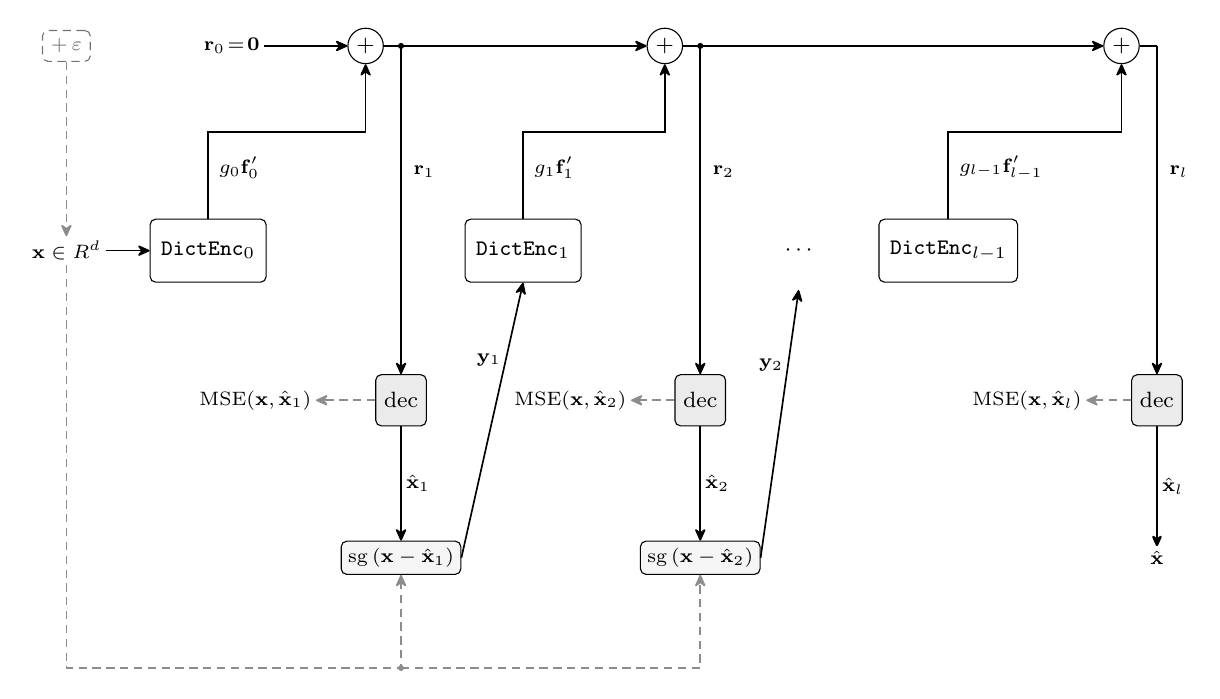
\begin{tikzpicture}[
    font=\footnotesize,
    >={Stealth[round,length=1.8mm,width=1.6mm]},
    blk/.style={draw, rounded corners=2pt, align=center,
                minimum height=8mm, inner xsep=4pt},
    hook/.style={draw, rounded corners=2pt, densely dashed, align=center,
                 inner sep=3pt, font=\scriptsize, black!55},
    dec/.style={draw, rounded corners=2pt, fill=black!8,
                minimum height=6.5mm, inner xsep=3pt},
    cond/.style={draw, rounded corners=2pt, fill=black!4, align=center,
                 inner sep=2.5pt, font=\scriptsize},
    add/.style={draw, circle, minimum size=4.5mm, inner sep=0pt},
    lab/.style={inner sep=1.5pt, font=\scriptsize},
    sig/.style={->, semithick},
    aux/.style={->, densely dashed, semithick, black!45},
  ]

  %% ---- layer row --------------------------------------------------
  \node[lab] (x)  at (-1.5,0) {$\mathbf{x}\in\mathbb{R}^{d}$};
  \node[blk] (D0) at ( 0.3,0) {$\mathtt{DictEnc}_0$};
  \node[blk] (D1) at ( 4.3,0) {$\mathtt{DictEnc}_1$};
  \node      (Dd) at ( 7.8,0) {$\cdots$};
  \node[blk] (DL) at ( 9.7,0) {$\mathtt{DictEnc}_{l-1}$};

  \draw[sig] (x) -- (D0);

  \node[hook] (noise) at (-1.5,2.6) {$+\,\varepsilon$};
  \draw[aux] (noise) -- (x);

  %% ---- residual accumulator (top rail, y = 2.6) --------------------
  \node[add] (A0) at ( 2.3,2.6) {$+$};
  \node[add] (A1) at ( 6.1,2.6) {$+$};
  \node[add] (AL) at (11.9,2.6) {$+$};

  \node[lab] (R0) at (0.6,2.6) {$\mathbf{r}_0\!=\!\mathbf{0}$};
  \draw[sig]      (R0) -- (A0);
  \draw[sig]      (A0) -- (A1);
  \draw[sig]      (A1) -- (AL);
  \draw[semithick] (AL) -- (12.35,2.6);

  %\node[lab] at (8.9,3.05) {$\mathbf{r}\in\mathbb{R}^{e}$: residual accumulator};

  %% ---- per-layer contributions g_l f'_l (enter from below) ----------
  \draw[sig] (D0.north) -- ++(0,1.1) -| (A0.south);
  \draw[sig] (D1.north) -- ++(0,1.1) -| (A1.south);
  \draw[sig] (DL.north) -- ++(0,1.1) -| (AL.south);
  \node[lab,anchor=west] at (0.38,1.05) {$g_0\mathbf{f}'_0$};
  \node[lab,anchor=west] at (4.38,1.05) {$g_1\mathbf{f}'_1$};
  \node[lab,anchor=west] at (9.78,1.05) {$g_{l-1}\mathbf{f}'_{l-1}$};

  %% ---- shared decoder, one decode per prefix -----------------------
  \node[dec] (Y1) at ( 2.75,-1.9) {$\mathrm{dec}$};
  \node[dec] (Y2) at ( 6.55,-1.9) {$\mathrm{dec}$};
  \node[dec] (YL) at (12.35,-1.9) {$\mathrm{dec}$};

  \draw[sig] ( 2.75,2.6) -- (Y1.north);
  \draw[sig] ( 6.55,2.6) -- (Y2.north);
  \draw[sig] (12.35,2.6) -- (YL.north);
  \fill ( 2.75,2.6) circle (1.1pt);
  \fill ( 6.55,2.6) circle (1.1pt);

  \node[lab,anchor=west] at ( 2.85,1.0) {$\mathbf{r}_1$};
  \node[lab,anchor=west] at ( 6.65,1.0) {$\mathbf{r}_2$};
  \node[lab,anchor=west] at (12.45,1.0) {$\mathbf{r}_{l}$};

  %% ---- deep supervision --------------------------------------------
  \node[lab] (L1) at ( 0.9,-1.9) {$\mathrm{MSE}(\mathbf{x},\hat{\mathbf{x}}_1)$};
  \node[lab] (L2) at ( 4.9,-1.9) {$\mathrm{MSE}(\mathbf{x},\hat{\mathbf{x}}_2)$};
  \node[lab] (LL) at (10.7,-1.9) {$\mathrm{MSE}(\mathbf{x},\hat{\mathbf{x}}_{l})$};
  \draw[aux] (Y1.west) -- (L1);
  \draw[aux] (Y2.west) -- (L2);
  \draw[aux] (YL.west) -- (LL);

  %% ---- residual forwarding ------------------------------------------
  \node[cond] (C1) at (2.75,-3.9)
  {$\mathrm{sg}\,(\mathbf{x}-\hat{\mathbf{x}}_1)$};
  \node[cond] (C2) at (6.55,-3.9)
  {$\mathrm{sg}\,(\mathbf{x}-\hat{\mathbf{x}}_2)$};
  \draw[sig] (Y1) -- node[right,lab]{$\hat{\mathbf{x}}_1$} (C1);
  \draw[sig] (Y2) -- node[right,lab]{$\hat{\mathbf{x}}_2$} (C2);

  \draw[sig] (C1.east) -- node[left,lab,pos=0.72]{$\mathbf{y}_1$} (D1.south);
  \draw[sig] (C2.east) -- node[left,lab,pos=0.72]{$\mathbf{y}_2$} (7.8,-0.5);

  %% ---- model output --------------------------------------------------
  \node[lab] (out) at (12.35,-3.9) {$\hat{\mathbf{x}}$};
  \draw[sig,thick] (YL) -- node[right,lab]{$\hat{\mathbf{x}}_{l}$} (out);

  %% ---- x broadcast to every conditioning step -------------------------
  \draw[aux] (x.south) -- (-1.5,-5.3) -- (2.75,-5.3) -- (C1.south);
  \draw[aux] (2.75,-5.3) -- (6.55,-5.3) -- (C2.south);
  \fill[black!45] (2.75,-5.3) circle (1.1pt);

\end{tikzpicture}

}
\caption[\texttt{Ontologizer} architecture]{\textbf{\texttt{Ontologizer} architecture.}
	An \texttt{Ontologizer} consists of $l$ stacked \texttt{DictEnc} layers.
	Each returns a pooled feature vector $\mathbf{f}'_\ell\in\mathbb{R}^{e}$,
	which is written, scaled by its input's gain $g_\ell$, to a residual
	accumulator $\mathbf{r}$.
	Layers are indexed $\ell = 0, \dots, l-1$ and accumulator states by the
	number of layers applied: $\mathbf{r}_0 := \mathbf{0}$ and
	$\mathbf{r}_{\ell+1} = \mathbf{r}_\ell + g_\ell\,\mathbf{f}'_\ell$, so
	layer $\ell$ reads state $\ell$ and writes state $\ell+1$; a stop-gradient
	variant ($\mathrm{sg}$ on $\mathbf{r}_\ell$, available but off in every model
	reported here) would prevent gradient communication between layers.
	$\mathrm{dec}$ is a linear decoder with shape $\mathbb{R}^{d \times e}$,
	shared by all layers.
	Deep supervision makes the code a successive refinement, coarse-to-fine
	in distortion as in residual quantizers~\cite{zeghidour2021} and
	nested-prefix SAEs~\cite{bussmann2025}: the component encoded by
	previous layers is inaccessible to later layers.
	After $\ell$ layers, $\hat{\mathbf{x}}_\ell = \mathrm{dec}(\mathbf{r}_\ell)$, and
	the component left unexplained is
	$\mathbf{y}_\ell = \mathbf{x} - \hat{\mathbf{x}}_\ell$, so $\mathbf{y}_0 = \mathbf{x}$.
	Layer $\ell$ classifies the shape of its input,
	$\mathbf{u}_\ell
	  = \mathbf{y}_\ell / \mathrm{L2}(\mathbf{y}_\ell) \oplus [1]$, and scales
	what it writes by the gain $g_\ell = \mathrm{L2}(\mathbf{y}_\ell)$.
	Normalizing prevents exploding gradients from repeated
	application of bilinear layers, each of which scales its input by
	$\lVert\cdot\rVert^{2}$; the constant coordinate keeps the sign of
	$\mathbf{y}_\ell$, which the bilinear form would otherwise lose.
	$\mathrm{MSE}(\mathbf{x},\hat{\mathbf{x}}_\ell)$ is computed separately for
	each prefix $\ell = 1, \dots, l$. The input-noise hook drawn on $\mathbf{x}$ is disabled in
	every model reported here.
}
\label{fig:onto-stack}
\end{figure}

\subsubsection{Classifier}
\label{sec:bilinear}
Each $\dictenc$'s classifier is a multihead bilinear map
($\bilinearblock$) with weights
$[\mathsf{W}, \mathsf{V}] \in \mathbb{R}^{2 \times h \times k \times d}$
($d+1$ with the constant coordinate of Equation~\ref{eq:y_norm}). It
reads the shape $\mathbf{u}_\ell$ of the layer's input (the residual left
by the layers before it, or $\mathbf{x}$ at layer 0), written $\mathbf{x}$
below for a generic input, and returns logits $K \in \mathbb{R}^{h \times k}$,
\begin{equation}
	\bilinearblock([\mathsf{W},\mathsf{V}],\mathbf{x}) :=
	\left(\sum^{d}_{q=1}W_{\cdot\cdot q}\,x_q\right)
	 \odot \left(\sum^{d}_{q=1}V_{\cdot\cdot q}\,x_q\right).
	 \label{eq:bilinearblock}
\end{equation}
Each logit is a quadratic form in $\mathbf{x}$, the low-rank form of
bilinear classifiers~\cite{pirsiavash2009,kim2017}, so a classifier admits
closed-form eigendecomposition in the manner of bilinear
MLPs~\cite{pearce2025}.

\begin{figure}[tp]
\centering
\resizebox{\linewidth}{!}{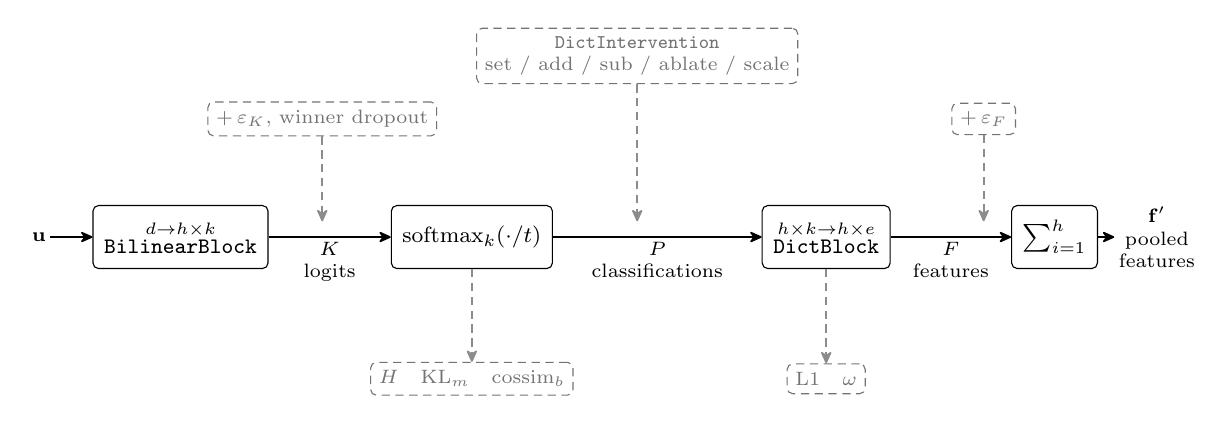
\begin{tikzpicture}[
    font=\footnotesize,
    >={Stealth[round,length=1.8mm,width=1.6mm]},
    blk/.style={draw, rounded corners=2pt, align=center,
                minimum height=8mm, inner xsep=4pt},
    hook/.style={draw, rounded corners=2pt, densely dashed, align=center,
                 inner sep=3pt, font=\scriptsize, black!55},
    lab/.style={inner sep=1.5pt, font=\scriptsize, align=center},
    sig/.style={->, semithick, align=center},
    aux/.style={->, densely dashed, semithick, black!45},
  ]

  %% ---- main chain ----------------------------------------------------
  \node[lab] (E)  at (-0.6,0) {$\mathbf{u}$};
  \node[blk] (CL) at ( 1.2,0) {$\bilinearblock^{d \to h \times k}$};
  \node[blk] (SM) at ( 4.9,0) {$\mathrm{softmax}_k(\cdot/t)$};
  \node[blk] (DB) at ( 9.4,0) {$\dictblock^{h \times k \to h \times e}$};
  \node[blk] (SU) at (12.3,0) {$\sum^{h}_{i=1}$};
  \node[lab] (F)  at (13.6,0) {$\mathbf{f}'$\\ pooled\\ features};

  \draw[sig] (E)  -- (CL);
  \draw[sig] (CL) -- node[below,lab]{$K$\\ logits}   (SM);
  \draw[sig] (SM) -- node[below,lab]{$P$\\ classifications}   (DB);
  \draw[sig] (DB) -- node[below,lab]{$F$\\ features} (SU);
  \draw[sig] (SU) -- (F);

  %% ---- training-time hooks and the intervention interface (above) ----
  \node[hook] (nk) at (3.0,1.5) {$+\,\varepsilon_K$,\ winner dropout};
  \node[hook] (iv) at (7.0,2.3) {\texttt{DictIntervention}\\
                                 set / add / sub / ablate / scale};
  \node[hook] (nf) at (11.4,1.5) {$+\,\varepsilon_F$};
  \draw[aux] (nk) -- (3.0,0.20);
  \draw[aux] (iv) -- (7.0,0.20);
  \draw[aux] (nf) -- (11.4,0.20);

  %% ---- where each regulariser attaches (below) -----------------------
  \node[hook] (lp) at (4.9,-1.8)
    {$H$\quad $\mathrm{KL}_m$\quad $\mathrm{cossim}_b$};
  \node[hook] (lf) at (9.4,-1.8)
    {$\mathrm{L1}$\quad $\omega$};
  \draw[aux] (SM.south) -- (lp);
  \draw[aux] (DB.south) -- (lf);

\end{tikzpicture}

}
\caption[\texttt{DictEnc} architecture]{\textbf{\texttt{DictEnc} architecture.}
	Dashed lines above indicate perturbations to the data,
	including noising and causal interventions.
	Dashed lines below indicate statistics used as tuneable auxiliary loss
	functions. Each \texttt{DictEnc} consists of a multihead bilinear
	classifier (§\ref{sec:bilinear}) and a multihead dictionary
	(§\ref{sec:dict}). Noise $\varepsilon_K$ and $\varepsilon_F$ and winner
	dropout regularize training (§\ref{sec:noise}).
	Assignments $P$ are $\mathrm{softmax}_{k}(K/t)$, or its straight-through
	argmax (§\ref{sec:labels}); interventions act on $P$. From $P$ we
	collect per-sample entropy $H$, between-sample similarity
	$\mathrm{cossim}_b$ and batch-mean entropy $\mathrm{KL}_m$
	(Equations~\ref{eq:entropy}--\ref{eq:KL}). A $\dictblock$ maps
	$P \in \mathbb{R}^{h \times k}$ to features
	$F \in \mathbb{R}^{h \times e}$ (Equation~\ref{eq:dictblock}); from $P$
	and the atoms we collect the support overlap $\omega$
	(Equation~\ref{eq:support}), and from $F$ the sparsity penalty
	$\mathrm{L1}$. $F$ is summed over heads to give pooled
	features $\mathbf{f}' \in \mathbb{R}^{e}$, which are added to the
	accumulator $\mathbf{r}$.
}
\label{fig:dictenc}
\end{figure}

\subsubsection{Assignments and selection}
\label{sec:labels}
Soft assignments are $P = \mathrm{softmax}_{k}(K/t)$, where the
temperature $t$ is annealed to sharpen them. A soft code's argmax is
not, however, what the model decodes: Section~\ref{sec:prelim-pareto}
finds the softmax model's discrete reading far from its embedding, as a
soft relaxation of quantization trained from scratch need not quantize
when the decoder can learn to invert it~\cite{vandenoord2017}. The
\emph{straight-through} selection rule makes the discrete code the model:
the forward pass selects the one-hot argmax, and the backward pass uses
$\mathrm{softmax}(K/t)$ as its surrogate gradient, the straight-through
estimator~\cite{bengio2013} in its categorical form~\cite{jang2017}. A
hard code transmits exactly $l\,h\log_2 k$ bits, and its only continuous
numbers are the layers' gains $g_\ell$.

From the assignments $P_n$ of each sample $n$ we collect per-sample
entropy, in bits,
\begin{equation}
	\mathrm{entropy}_k(P)_i :=
	-\sum^{k}_{j=1}p_{ij}\log_2 p_{ij},
	\qquad
	H := \mathbb{E}_{n}\,\mathbb{E}_{i}\!\left[
	\mathrm{entropy}_k(P_n)_i\right],
	\label{eq:entropy}
\end{equation}
between-sample similarity, the mean absolute cosine of the per-head
features over pairs of samples, with
$\cos\angle(\mathbf{a}, \mathbf{b}) :=
\langle\mathbf{a},\mathbf{b}\rangle / (\lVert\mathbf{a}\rVert\lVert\mathbf{b}\rVert)$
the cosine of the angle between two vectors, evaluated through each
head's dictionary Gram $G_i = \lvert D_{i}\rvert \lvert D_{i}\rvert^{\top}$,
\begin{equation}
	\mathrm{cossim}_b :=
	\mathbb{E}_{n,n'}\big\lvert
	\cos\angle(\mathbf{f}_{n}, \mathbf{f}_{n'})
	\big\rvert,
	\qquad
	\langle \mathbf{f}_{n}, \mathbf{f}_{n'}\rangle
	= \sum^{h}_{i=1}\mathbf{p}_{ni}^{\top}G_{i}\,\mathbf{p}_{n'i},
	\label{eq:cossim_b}
\end{equation}
and the divergence of the batch-mean assignment from uniform,
\begin{equation}
	\mathrm{KL}_m := \mathbb{E}_{i}\!\left[\log_2 k -
	\mathrm{entropy}_k\!\left(\mathbb{E}_n[P_n]\right)_i\right].
	\label{eq:KL}
\end{equation}
$\mathrm{KL}_m$ anchors each head's mean assignment to uniform, which
keeps every entry in use.

\subsubsection{Dictionary}
\label{sec:dict}
A $\dictblock$ with weights $\mathsf{D} \in \mathbb{R}^{h \times k \times e}$
maps assignments to per-head features $F \in \mathbb{R}^{h \times e}$,
whose row $\mathbf{f}_i$ is head $i$'s output,
\begin{equation}
	\mathbf{f}_i :=
	\sum^{k}_{j=1} p_{ij}\,\mathbf{a}_{ij},
	\qquad
	\mathbf{a}_{ij} := \lvert \mathsf{D}_{ij\cdot}\rvert .
	\label{eq:dictblock}
\end{equation}
Atoms are non-negative and assignments lie on the simplex, so features
are strictly additive and each head's output lies in the convex hull of
its atoms (Figure~\ref{fig:head-simplex}).

\begin{figure}[tp]
\centering
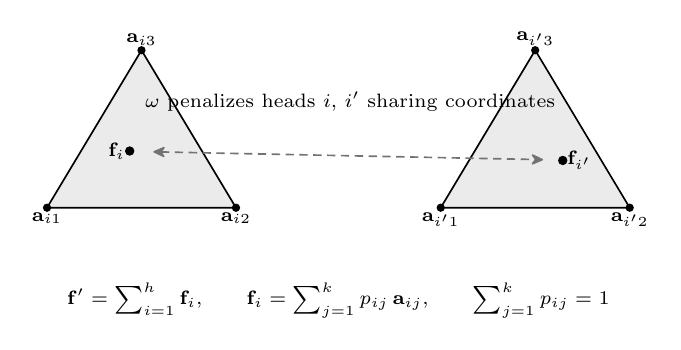
\begin{tikzpicture}[
    font=\footnotesize,
    >={Stealth[round,length=1.8mm,width=1.6mm]},
    lab/.style={inner sep=1.5pt, font=\scriptsize},
  ]
  %% ---- head i --------------------------------------------------------
  \fill[black!8]   (0,0) -- (2.4,0) -- (1.2,2.0) -- cycle;
  \draw[semithick] (0,0) -- (2.4,0) -- (1.2,2.0) -- cycle;
  \fill (0,0)     circle (1.5pt) node[below,lab]{$\mathbf{a}_{i1}$};
  \fill (2.4,0)   circle (1.5pt) node[below,lab]{$\mathbf{a}_{i2}$};
  \fill (1.2,2.0) circle (1.5pt) node[above,lab]{$\mathbf{a}_{i3}$};
  \fill (1.05,0.72) circle (1.7pt) node[left,lab]{$\mathbf{f}_i$};

  %% ---- head i' ------------------------------------------------------
  \fill[black!8]   (5.0,0) -- (7.4,0) -- (6.2,2.0) -- cycle;
  \draw[semithick] (5.0,0) -- (7.4,0) -- (6.2,2.0) -- cycle;
  \fill (5.0,0)   circle (1.5pt) node[below,lab]{$\mathbf{a}_{i'1}$};
  \fill (7.4,0)   circle (1.5pt) node[below,lab]{$\mathbf{a}_{i'2}$};
  \fill (6.2,2.0) circle (1.5pt) node[above,lab]{$\mathbf{a}_{i'3}$};
  \fill (6.55,0.60) circle (1.7pt) node[right,lab]{$\mathbf{f}_{i'}$};

  \draw[<->, densely dashed, semithick, black!55] (1.35,0.71) -- (6.30,0.61);
  \node[lab] at (3.85,1.35)
    {$\omega$ penalizes heads $i$, $i'$ sharing coordinates};

  \node[lab, anchor=north, align=center] at (3.7,-0.9)
  {$\mathbf{f}'=\sum^h_{i=1} \mathbf{f}_i$,\qquad
  $\mathbf{f}_i=\sum^k_{j=1} p_{ij}\,\mathbf{a}_{ij}$,\qquad $\sum^k_{j=1} p_{ij}=1$};
\end{tikzpicture}


\caption[Per-head geometry]{\texttt{DictBlock} \textbf{head geometry} for $h{=}2$; $k{=}3$.
	The output space of a head $i$ is a simplex with its atoms
	$\mathbf{a}_{ij}$, the rows of $\lvert D_i\rvert$, as vertices. The assignment $P$ is a soft
	choice among mutually contrastive categories rather than a set of
	independently firing features, and because $p_{ij} \in [0,1]$ the
	output lies within the convex hull of the head's atoms.
	Because $\lvert \mathsf{D}\rvert\geq0$ and $P\geq0$, $F\geq0$, so
	$\cos\angle(\mathbf{f}_i, \mathbf{f}_{i'}) \in [0,1]$, and driving the support overlap $\omega$
	to zero asks the heads to partition the coordinates of $\mathbb{R}^e$
	between them (§\ref{sec:disjoint}).
}
\label{fig:head-simplex}
\end{figure}

\paragraph{Disjoint support}
\label{sec:disjoint}
For non-negative vectors the inner product is a sum of non-negative
terms, so it vanishes exactly when the supports are disjoint,
\begin{equation}
	\langle \mathbf{u},\mathbf{v}\rangle = 0
	\iff
	\mathrm{supp}(\mathbf{u}) \cap \mathrm{supp}(\mathbf{v}) = \emptyset .
	\label{eq:disjoint}
\end{equation}
Between heads, then, orthogonality is not a rotation constraint but a
support partition. The support overlap compares heads' usage-weighted
coordinate profiles,
\begin{equation}
	\boldsymbol{\pi}_i := \sum^{k}_{j=1} \bar{p}_{ij}\,
	\lvert \mathbf{a}_{ij}\rvert,
	\qquad
	\omega := \mathbb{E}_{i \neq i'}\,
	\frac{\langle \boldsymbol{\pi}_i, \boldsymbol{\pi}_{i'}\rangle}
	     {\lVert \boldsymbol{\pi}_i\rVert \lVert \boldsymbol{\pi}_{i'}\rVert},
	\qquad
	\bar{\mathbf{p}}_i := \mathbb{E}_{n}\,[\mathbf{p}_{ni}],
	\label{eq:support}
\end{equation}
and is zero exactly when no two heads share a coordinate. Because a
softmax gives every entry positive weight, a single sample on which two
heads are orthogonal forces every pair of their atoms to be disjoint:
the partition is a property of $\mathsf{D}$, holding for all inputs,
which is the premise a static reading of the dictionary needs.
With concatenated heads, heads write disjoint
slices by construction and $\omega$ is identically zero.

Two orthogonalities are in play. Disjoint support assigns each head a
block of coordinates; \emph{within} a head the $k$ atoms are contrastive
alternatives spread apart inside that block, which
Section~\ref{sec:prelim-orth} measures. Neither is guaranteed at
convergence: $\omega$ is a penalty, and the geometry makes a support
partition the cheap solution rather than forcing one. Measured, the
within-head orthogonality holds and the between-head partition does not
form (Section~\ref{sec:prelim-orth}).

\subsubsection{Decoder}
\label{sec:decoder}
Each layer's pooled output $\mathbf{f}'_\ell = \sum_{i=1}^{h}\tilde{\mathbf{f}}_{i}$ is scaled
by its input's gain $g_\ell$ and added to the accumulator, whose state
after $\ell$ layers a single unbiased linear map shared by all layers
decodes,
\begin{equation}
	\mathbf{r}_\ell = \sum_{\ell'=0}^{\ell-1} g_{\ell'}\,\mathbf{f}'_{\ell'},
	\qquad
	\hat{\mathbf{x}}_\ell = W_{\mathrm{dec}}\mathbf{r}_\ell,
	\qquad
	W_{\mathrm{dec}} \in \mathbb{R}^{d \times e}.
	\label{eq:dec}
\end{equation}
The residual $\mathbf{y}_\ell$, layer $\ell$'s input, is stop-gradiented,
so that lower layers cannot write a communication code into it instead
of reducing it, and split into a gain and a shape $\mathbf{u}_\ell$, its
unit direction with a constant coordinate appended, which is what layer
$\ell$ classifies:
\begin{equation}
	\mathbf{y}_\ell = \mathrm{sg}\!\left[\mathbf{x} - \hat{\mathbf{x}}_\ell\right],
	\qquad
	\mathbf{u}_\ell =
	\frac{\mathbf{y}_\ell}{\mathrm{L2}(\mathbf{y}_\ell) + \epsilon} \oplus [1],
	\qquad
	g_{\ell} := \mathrm{sg}\!\left[\mathrm{L2}(\mathbf{y}_\ell)\right].
	\label{eq:y_norm}
\end{equation}
The empty sum makes $\mathbf{r}_0 = \mathbf{0}$, so $\mathbf{y}_0 = \mathbf{x}$:
layer 0 classifies the input itself.
Under \texttt{resid\_gain} each layer classifies the direction of what it
corrects, and the gain carries the magnitude it cannot see; without it
$g_\ell = 1$.

\paragraph{Direct atoms and fibers.}
Two variants change what an entry writes. With \emph{direct atoms} the
dictionary is signed and lives in the output space itself, with no
decoder, so every atom is literally a steering direction. With
\emph{fibers} each entry carries a rank-$r$ local basis, and each head
reads $r$ coordinates from its input, so a hard code becomes a discrete
base point plus a continuous correction within that entry's fiber;
training the fibers after freezing the base keeps the discrete code
exactly what it was.

\subsubsection{Noise and dropout}
\label{sec:noise}
Classifier logits take Gaussian noise $\varepsilon_K$, relative to the
logit scale under a hard forward; features take noise $\varepsilon_F$
proportional to each feature's batch standard deviation, stop-gradiented
so the model cannot evade it by shrinking variance. Winner dropout sets a
head's argmax logit to $-\infty$ with probability $p_{\mathrm{drop}}$.

\subsection{Training}
\label{sec:training}

\subsubsection{Embedding model}
\label{sec:sonar}
We embed texts using SONAR~\cite{sonar}, a multimodal and
language-agnostic sentence embedding model: a translation-trained
encoder, mean-pooled into one 1024-dimensional vector, and a decoder that
generates text from that vector alone, in a target language chosen at
decoding time. Translations embed close together, so a reconstructed or
steered embedding can be decoded in one fixed language and re-encoded,
which is how text fidelity and text-cycle steering are scored. Large
Concept Models~\cite{lcmteam2024largeconceptmodelslanguage} generate one
sentence embedding per step in SONAR space, so an edit to a SONAR
embedding is an edit to an LCM's context or output; the same work finds
SONAR decoding fragile to small perturbations. GPT-2 small's residual
stream~\cite{radford2019} is a second
substrate, where sparse dictionary learning is known to work and the
reconstruction can be spliced back into the model.

\subsubsection{Loss function}
\label{sec:loss}
Reconstruction is trained with a whitened MSE, $\mathbf{w}$ being the
per-dimension inverse variance normalized to mean one,
\begin{equation}
	\mathrm{MSE}(X,\hat{X}) := \frac{1}{bd}\sum^{b}_{n=1}\sum^{d}_{q=1}
	w_q\left(\hat{x}_{nq} - x_{nq}\right)^2,
	\label{eq:mse}
\end{equation}
under deep supervision~\cite{lee2015deeply}: it is computed at every prefix
$\hat{X}_\ell$, $\ell = 1, \dots, l$, and averaged, so each layer must explain
what earlier layers left unexplained. The auxiliary statistics are weighted
and summed over layers,
\begin{equation}
	L := \frac{1}{l}\sum^{l}_{\ell=1}\mathrm{MSE}(X,\hat{X}_\ell)
	+ \sum^{l-1}_{\ell=0}\mathbf{s}\cdot\boldsymbol{\psi}_\ell,
	\qquad
	\boldsymbol{\psi}_\ell := \big[\, \mathrm{L1} \;\; \mathrm{cossim}_b \;\;
	\mathrm{KL}_m \;\; \omega \,\big]^{\top}_\ell,
	\label{eq:loss_total}
\end{equation}
with $\mathrm{L1}$ the batch mean of each sample's feature norm. In
practice $\mathrm{cossim}_b$ also minimizes $H$, which therefore carries
no weight. Most models reported here trained before $\omega$ existed, with
its predecessor in that slot (the mean cosine between heads' features
within a sample); a direct $\omega$-penalty sweep on GPT-2 is reported in
Section~\ref{sec:prelim-orth}.

\subsection{Evaluation}
\label{sec:eval}
Evaluation runs against $\topk$ SAEs~\cite{gao2024} trained on the same
cached embeddings under the same whitened objective, scored by whitened
fraction of variance unexplained ($\mathrm{FVU}_w$) on a held-out tail.
A structural-ablation ladder of SAE variants adds one Ontologizer
commitment at a time; two of its rungs, which add per-head competition
over a shared decoder, are one-layer Ontologizers with linear
classifiers (\texttt{g160top1} with hard selection, \texttt{g160softmax}
with softmax) and are reported as simplified variants rather than
baselines. The headline instruments are reconstruction against code
capacity and a Gaussian rate--distortion reference~\cite{cover2006}; the
semantic coherence of a
head's decoded atoms against size-matched nulls; steering scored in
embedding space (whether a step realizes the target entry, and what
share of other heads it disturbs, against a random step of the same
length); additivity of paired interventions; cross-seed head matching
by partition and by contribution; and blinded auto-interpretability.
AxBench~\cite{wu2025axbenchsteeringllmssimple} found that prompting,
finetuning and one simple supervised direction, the difference of means,
beat SAE latents at steering, while a linear probe's direction did not;
the steering comparison here, which includes both, is built to face that
result.

\section{Preliminary results}
\label{sec:prelim}
The evaluation is in progress, and its results are mixed. This section
gives the headline of each line of work; the full methodology, the
eliminations behind each result and the supplementary measurements are
in the working notes\footnote{K.~Wiechecki et al., \emph{Dictionary
learning as unsupervised steering-vector generation: Ontologizers vs.\
sparse autoencoders on SONAR sentence embeddings}, working notes, in
preparation; distributed with this proposal.}.

Three models recur. The softmax Ontologizer \texttt{resid\_nc} has $l{=}5$
layers of $h{=}32$ heads with $k{=}32$ entries, a soft code. The
straight-through Ontologizer \texttt{ste\_h76\_init01} has $5\times76$
heads at $k{=}32$, a hard code of 1900 bits. The SAEs are $\topk$ SAEs
on the same cache and objective. The cache holds SONAR embeddings of an
86-language mC4 sample, 93\% of them encoded under SONAR's English source
tag rather than their own, which moves an embedding by about twice the
hard code's reconstruction error but changes how much of it language
explains only from 7.4\% to 6.7\%. Scores are $\mathrm{FVU}_w$ on the
final 32{,}768 cache rows, which the SAEs and the straight-through arms
never train on. The softmax Ontologizers predate that holdout, but their
scores move by at most 0.3\% on freshly encoded rows that no model saw.

\subsection{The price of a soft code}
\label{sec:prelim-pareto}
Contrast-set structure is expensive in a soft code. The plain-SAE
frontier dominates the softmax Ontologizer's deviation code (each head's
$\nu$ entries furthest from the mean assignment kept, the rest pinned to
it) at every capacity measured (Table~\ref{tab:prelim-pareto}): at
$\mathrm{FVU}_w \approx 0.49$ the SAE transmits 32 coefficients where the
Ontologizer needs 320, and at matched budgets an unstructured code
reconstructs about $50\times$ better. The soft model's own discrete
reading is not a code at all: its argmax lands $77\times$ above the least
distortion an 800-bit code could reach if the embeddings were Gaussian
with their covariance. Real data is no harder to compress than a Gaussian
of the same covariance~\cite{cover2006}, so that is a lower bound on its
distance from the least distortion any 800-bit code could reach on this
data (a limit approached by coding long blocks of samples jointly), and
the entries an intervention forces are not what carries the soft model's
embedding. That is the motivation for the hard code.

\begin{table}[tp]\centering\small
\begin{tabular}{@{}lrrr@{}}
\toprule
point & coeffs & index bits & $\mathrm{FVU}_w$ \\
\midrule
onto $\nu{=}0$ (mean-assignment origin) & 0 & 0 & 1.001 \\
onto hard (argmax)                  & 0 & 800 & 17.34 \\
\emph{Gaussian reference, 800 bits} & 0 & 800 & \emph{0.226} \\
SAE $k_{\mathrm{SAE}}{=}32$ tier    & 32 & 276--313 & 0.494--0.509 \\
onto dev $\nu{=}1$                  & 160 & 800 & 0.677 \\
SAE $k_{\mathrm{SAE}}{=}160$        & 160 & 1206 & 0.258 \\
onto dev $\nu{=}4$                  & 640 & 2421 & 0.289 \\
onto dev $\nu{=}8$                  & 1280 & 3732 & 0.094 \\
SAE $k_{\mathrm{SAE}}{=}5120$ ($\mathrm{L0}{\approx}1520$) & 1520 & 6423 & \textbf{0.00011} \\
1-layer soft variant \texttt{g160softmax} & 5120 & 0 & 0.00436 \\
onto soft ($\nu{=}32$)              & 5120 & 0 & 0.00538 \\
\bottomrule
\end{tabular}
\caption{Reconstruction against code capacity for the softmax
Ontologizer \texttt{resid\_nc}. Ontologizer points truncate each head to
its $\nu$ largest deviations from the mean assignment; SAE points use
measured $\mathrm{L0}$. Index bits name which coefficients are sent, as a
set: $l\,h\log_2\binom{k}{\nu}$ for the Ontologizer and
$\log_2\binom{m}{\mathrm{L0}}$ for an SAE of $m$ latents. The Gaussian reference is reverse water-filling on the
evaluation tail's whitened covariance~\cite[Thm.~10.3.3]{cover2006}: the least
distortion at that rate for a Gaussian source of that covariance, which
real data can beat.}
\label{tab:prelim-pareto}
\end{table}

\subsection{Heads are contrast sets}
\label{sec:prelim-orth}
Trained heads carry the signature the steering goal predicts. Every
entry has an exact decode direction in output space, and within a soft
head those directions repel: in 96\% of the softmax Ontologizer's heads
they are more dissimilar than size-matched random sets of atoms from the
same pool (Table~\ref{tab:prelim-headcoh}). A head holds well-separated
alternatives along one dimension, not a semantic cluster, and the
repulsion strengthens under the training objective's whitened inner
product. The hard code agrees from the weights: a head's decoded atoms
are orthogonal to slightly repelling (mean cosine $0.023$ at layer 0,
$-0.015$ to $-0.020$ below). Hard per-head selection in a single linear
layer gives the opposite signature, heads that tile one region.

The other orthogonality the architecture was designed for did not
emerge. No trained summed model partitions its dictionary space between
heads: the support overlap $\omega$ (Equation~\ref{eq:support}) sits at or
above a null that shuffles each head's coordinates, in every model
measured, and each head's usage covers 52--98\% of the coordinates where a
partition into 32 heads needs about 3\%. This holds for the part of each
atom the decoder sees as well as for its null-space part, and penalizing
$\omega$ directly on GPT-2 drives it down in the dictionary space only by
moving 73--95\% of atom energy into the decoder's null or near-null space,
while the decoded atoms stay 8--10\% above their null (working notes).
Summed heads are contrast sets that share their coordinates; concatenated
heads supply the partition by construction.

\begin{table}[tp]\centering\small
\begin{tabular}{@{}lrrrr@{}}
\toprule
heads or grouping & count & mean $\zeta_{\cos}$ & frac $\zeta{>}2$ & frac $\zeta{<}{-}2$ \\
\midrule
\texttt{g160top1} (trained, hard)   & 160 & $+161.3$ & 1.00 & 0.00 \\
$k_{\mathrm{SAE}}{=}32$ SAE, discovered groups & 359 & $+1.7$ & 0.36 & 0.02 \\
Ontologizer heads (trained, soft)   & 160 & $-17.6$ & 0.04 & \textbf{0.96} \\
\texttt{g160softmax} (trained, soft) & 160 & $-14.7$ & 0.00 & \textbf{1.00} \\
\bottomrule
\end{tabular}
\caption{Within-head decode-direction coherence $\zeta_{\cos}$,
standardized against size-matched same-pool nulls
($n_{\text{null}}{=}500$). Soft heads are
anti-coherent: their atoms are pushed apart.}
\label{tab:prelim-headcoh}
\end{table}

\subsection{A discrete code beats $\topk$ SAEs, not every sparse code}
\label{sec:prelim-ste}
Under straight-through selection the forward pass is the argmax, and the
discrete code is the model. At 1900 index bits the hard code reaches
$\mathrm{FVU}_w$ $0.154$. Its only continuous numbers are four
per-layer gains, and with those pinned to their means it is a pure
1900-bit code at $0.158$. A code that also sends coefficients reaches
that total only at some precision for them, and no coding of an SAE's
coefficients beats the least-squares fit on its own support. A $\topk$
SAE that names its 160 active latents in 1206 bits totals 1900 bits at
4.3 bits per coefficient, where its error is at least $0.236$, so at
matched total rate the pure code is at least $33\%$ below it
(Table~\ref{tab:prelim-ste}). An SAE whose sparsity is not fixed does
better: with every code's coefficients quantized and each slot's symbols
entropy-coded, an L1 SAE with a weak penalty reaches $0.129$ at 1900
bits averaged over rows, because its latents fire unevenly and are cheap
to name and its rows vary in length, while the hard code uses its
entries almost uniformly in a code of fixed length. Held to 1900 bits on
every row the L1 SAE reaches $0.152$, level with the hard code, and
charging every support its fixed-length cost, the hard code leads
($0.158$ against $0.180$). The stack sits $3.1\times$
above the Gaussian reference for its rate, so at least that far above
the data's distortion--rate function at 1900 bits, a long-block limit
that a code describing each sample alone need not
approach~\cite{cover2006}.

\begin{table}[tp]\centering\small\setlength{\tabcolsep}{4pt}
\begin{tabular}{@{}lrrrrr@{}}
\toprule
code & coeffs & index bits & $\mathrm{FVU}_w$ & at 1900 bits & every row \\
\midrule
\textbf{straight-through Ontologizer, $5\times76$} & \textbf{4 gains} & \textbf{1900} & \textbf{0.154} & \textbf{0.155} & --- \\
\quad gains pinned to their means & 0 & 1900 & 0.158 & --- & 0.158 \\
SAE, $\topk$, $k_{\mathrm{SAE}}{=}160$ & 160 & 1206 & 0.258 (0.236) & 0.259 & 0.258 \\
SAE, ReLU+L1 $3\times10^{-5}$ & 519 & 2418 & 0.219 & 0.242 & 0.250 \\
SAE, ReLU+L1 $10^{-5}$ & 1438 & 4380 & 0.048 & 0.175 & 0.200 \\
SAE, ReLU+L1 $3\times10^{-6}$ & 1637 & 4623 & 0.005 & \textbf{0.129} & \textbf{0.152} \\
1-layer hard variant \texttt{g160top1} & 160 & 800 & 0.274 (0.273) & 0.274 & 0.274 \\
\bottomrule
\end{tabular}
\caption{The hard code against converged SAEs on the held-out tail. In
parentheses, the least-squares fit on each code's own support, the least
error any coding of its coefficients can reach. ``At 1900 bits'' is each
code's error at a total of 1900 bits per sample averaged over rows, with
everything it sends quantized and each slot's symbols entropy-coded;
``every row'' holds each row to 1900 bits, the pinned hard code at fixed
length. \texttt{g160top1}
shares the hard per-head selection but has one layer of linear
classifiers and keeps a magnitude on each winner; its index bits name
each head's winner.}
\label{tab:prelim-ste}
\end{table}

\subsection{Depth helps reconstruction and costs addressability}
\label{sec:prelim-depth}
Five layers of 76 heads and one layer of 380 have the same bits and
exactly the same parameter count, and every head in both uses its entries
almost uniformly. The stack's
error is $1.79\times$ lower ($0.1535$ against $0.2750$), and the gain
comes from pairing each stage's input with the sample's own earlier
error: a flat layer decodes like an additive
quantizer~\cite{babenko2014}, but its heads choose in parallel rather
than each against what the others leave, so no head sees another's error
(harmless in a product quantizer~\cite{jegou2011}, whose heads own
disjoint coordinates, but not when atoms overlap), while the stack is a
residual quantizer~\cite{zeghidour2021}. The stack also trains each of its prefixes
to reconstruct, which a single layer cannot, and that difference is not
yet separated from the pairing.

The same cascade entangles the heads. A step in embedding space along a
target entry's decode direction, a quarter of the input's norm long,
realizes the target on 99.6\% of rows in the flat model while disturbing
33\% of the other heads; in the stack it realizes 37\% while disturbing
66\%. In both, every direction disturbs as many other heads as a random
step of the same length: the hard code's heads sit almost on their
decision boundaries (median winner--runner-up margin $1.5\times10^{-4}$),
and the cascade adds downstream layers reclassifying a changed residual.
The one Ontologizer whose decode direction avoids the other heads is
the simplest, \texttt{g160top1}: it realizes 58\% of targets while
disturbing $2.6\%$ of other heads, against $23\%$ for a random step.

\subsection{Steering}
\label{sec:prelim-steer}
Steering works when it is measured where it acts. In the soft model a
decode-direction step of a quarter of the input's norm realizes the
target entry on 82\% of rows, against 2\% for a random step of the same
length; the text
round trip had hidden this, since an unsteered decode--re-encode cycle
preserves a head's choice on only $11$--$13\%$ of rows. Interventions
set directly on a head compose: the decode change of a joint two-head
intervention points where the sum of the single interventions points
(median cosine at least $0.95$ in every layer, exact in the last, where
nothing downstream can reclassify). Forcing one first-layer entry of
\texttt{resid\_nc} reliably steers decodes into Burmese while preserving
their content, a causally verified existence proof on one seed.

Against supervised steering on the model's own categories in embedding
space (at $0.25\lVert\mathbf{x}\rVert$), the softmax stack's decode
direction reaches $75\%$ of targets against $46$--$47\%$ for
difference-of-means and logistic-probe vectors, while the hard stack's
decode direction reaches $37\%$ against $91$--$94\%$. Yet two
arbitrary-partition baselines show that reaching a partition's cells in
embedding space is a property of partitioning the space rather than
evidence that the learned partitions are meaningful: in an untrained
$5\times76$ stack, the parametric decode step is random ($2\%$), but the
supervised vectors ($75\%$ and $94\%$) and classifier gradients ($61\%$
and $85\%$, vs.\ $30\%$ and $16\%$ trained) reach its random cells at a
third of the trained stack's collateral ($22\%$ vs.\ $66\%$); and in
$1\times380$ random-projection heads ($k{=}32$), empirical cell-centroid
swaps reach $78\%$ ($67\%$ at native step) and the target projection
vector, margin gradient, and logistic probe reach $100\%$ ($87\%$ for
difference of means) at $30$--$32\%$ collateral, matching the trained flat
arm. Against supervised steering on an external concept, language, under
matched intervention budgets (Table~\ref{tab:steer-overlay}), forcing an
entry moves decodes along the supervised difference-of-means direction
$0.64\times$ as far as supervised steering itself and $4\times$ as far as
linear-probe directions. Every arm's collateral, supervised steering
included, sits at the random-direction floor.

\begin{table}[tp]\centering\small
\begin{tabular}{@{}lrrrr@{}}
\toprule
arm & eff (native) & eff (dm frame) & hit rate & collateral \\
\midrule
difference of means    & 0.474 & 0.474 & 0.062 & 0.752 \\
entry forcing          & 0.399 & 0.302 & 0.000 & 0.776 \\
linear probe           & 0.294 & 0.072 & 0.000 & 0.701 \\
random direction       & --    & --    & --   & 0.705 \\
\bottomrule
\end{tabular}
\caption{Language steering under matched intervention budgets on the
softmax Ontologizer \texttt{resid\_nc\_hm}; medians over 24
language--magnitude conditions per arm. Effect is displacement along the
arm's own direction (native) and along the shared difference-of-means
direction (dm frame); hit rate is the fraction of steered decodes
reaching the median projection of genuine target-language rows;
collateral is content change elsewhere, with the random direction as its
floor.}
\label{tab:steer-overlay}
\end{table}

\subsection{The error reproduces; the heads do not}
\label{sec:prelim-seed}
Two hard-code runs differing only in seed reach identical held-out error,
$0.1535$ and $0.1535$. Nothing that identifies an individual head
agrees: matched head partitions score a mean NMI of $0.012$ against a
$0.005$ null, and head contributions a centered cosine of $0.007$
against $0.002$, while a run against its own earlier checkpoint scores
$0.38$ on partitions. Nor do the two seeds compute one reconstruction:
their whitened residuals correlate at $0.30$, where the two seeds of a
$k_{\mathrm{SAE}}{=}32$ SAE reach $0.83$. Within one run each head keeps
its atoms (cosine $0.98$--$0.99$ to its own checkpoint 19{,}500 steps
earlier), so what fails is replication across seeds, not stability in
training. GPT-2 replicates the pattern: only the first
layer reproduces, at under a fifth of a same-run control. The softmax
Ontologizer fares no better, matching at most $0.1\%$ of entries across
seeds where the $k_{\mathrm{SAE}}{=}32$ SAE pair matches 3--31\%. The first layer is the
only one whose input does not depend on upstream choices, and one head
in it does recur: the strongest head in every run, found at different
indices in different seeds, encodes topic and genre (its entries decode
to crime news, geopolitics, encyclopedic description, manufacturing,
marketing, legislation and entertainment, and contrastive descriptions
of them are detected at F1 $0.52$ against a $0.27$ null). Language, the
corpus's one labelled factor, is carried as neighbourhoods across heads
and never by one, as a language-agnostic embedding should give.

\subsection{Hard codes on GPT-2}
\label{sec:prelim-gpt2}
On GPT-2 small, with signed atoms in activation space and no decoder, an
800-bit hard code recovers more of the model's loss when its
reconstruction is spliced back in than a $k_{\mathrm{SAE}}{=}32$ SAE both
on the same 10M-token training cache ($97.0\%$ vs.\ $96.2\%$, at
$\mathrm{FVU}$ $0.217$ vs.\ $0.189$) and after one pass over 40M tokens
($97.6\%$ at $0.195$; Table~\ref{tab:prelim-gpt2}), though with its 32
coefficients quantized to $\sim$5 bits each (556--588 total bits against
$800 + {\sim}25$) the SAE leads on FVU per bit; across architectures,
$\mathrm{FVU}$ does not order downstream loss. Giving the 40M
concatenated-head model per-layer decoders cuts $\mathrm{FVU}$ from
$0.186$ to $0.169$ ($97.3\% \to 97.7\%$ recovered) and drops cross-layer
same-head coupling from $97\%$ to $6\%$ (chance $3\%$; a width-matched
shared decoder control is still owed). Fibers trained on top of the frozen
discrete code recover $99.9\%$ while leaving the code exactly as it was,
at the price of 640 continuous numbers per token.

\begin{table}[tp]\centering\small
\begin{tabular}{@{}llrr@{}}
\toprule
model & code per token & $\mathrm{FVU}$ & loss recovered \\
\midrule
hard code, direct atoms (10M tokens) & 800 bits + 5 gains & 0.217 & 97.0\% \\
\textbf{hard code, direct atoms (40M tokens)} & 800 bits + 5 gains & 0.195 & \textbf{97.6\%} \\
hard code, concatenated heads & 800 bits + 5 gains & 0.186 & 97.5\% \\
hard code, concatenated heads, $k{=}64$ & 960 bits + 5 gains & \textbf{0.164} & \textbf{97.9\%} \\
$\topk$ SAE, $k_{\mathrm{SAE}}{=}32$ & 32 coeffs + $\sim$276 bits & 0.189 & 96.2\% \\
$\topk$ SAE, $k_{\mathrm{SAE}}{=}128$ & 128 coeffs + $\sim$859 bits & 0.116 & 98.6\% \\
\bottomrule
\end{tabular}
\caption{GPT-2 small, residual stream entering block 8, held-out
documents. Loss recovered is
$(\mathrm{CE}_{\mathrm{ablate}} - \mathrm{CE}_{\mathrm{recon}}) /
(\mathrm{CE}_{\mathrm{ablate}} - \mathrm{CE}_{\mathrm{clean}})$ with the
residual mean-ablated as the floor; FVU is unwhitened here. Concatenated
heads write disjoint 48-dimensional blocks through a shared decoder. SAEs
train 10 epochs over the 10M-token cache (556--588 total bits for
$k_{\mathrm{SAE}}{=}32$ at $\sim$5 bits per coefficient). One seed per
Ontologizer (10M direct seed-43 replica: $\mathrm{FVU}$ $0.219$, $96.9\%$).}
\label{tab:prelim-gpt2}
\end{table}

On these GPT-2 codes, describability and steering each add a caution.
Blinded LLM-judged detection of entry descriptions (balanced accuracy;
chance $0.50$, document-split nulls $0.496$--$0.507$) drops sharply with
depth: layer~0 averages $0.70$--$0.71$ ($0.91$ on top members, $0.65$ on
random members, $0.55$ near the boundary), layer~1 falls to $0.56$--$0.57$,
and layers~2--4 sit at the $0.50$--$0.52$ null; in layer~0 a rule that sees
only token identity beats the judge on single cells ($0.75$ vs.\ $0.69$ on
concatenated heads, $0.74$ vs.\ $0.71$ on direct atoms), and two-head
chains add $+0.10$ on concatenated heads mostly from lexical information
($+0.01$ on direct). Single-head edits are small in next-token KL (setting
a layer-0 head to its mean entry costs $0.02$--$0.075$ nats vs.\ $0.055$
for zeroing an active SAE latent; entry swaps cost $0.001$--$0.06$ nats),
and swapping a head to entry $j'$ steers the next-token distribution
specifically toward $j'$'s empirical distribution (mean rank $3.5$--$6$ of
31 at unit step and $5$--$8$ at $4\times$, vs.\ $14$--$18$ for random
directions). Yet centroid steps between random-projection bins steer just
as specifically in every layer (mean rank $0.21$--$1.69$ across layers
0--4 vs.\ $0.56$--$1.37$ for learned cells), because the downstream map to
the logits is locally close to linear.

\subsection{Automated interpretability}
\label{sec:prelim-autointerp}
Per-latent lenses mis-measure classifier codes, whose content lives in
partitions rather than latent magnitudes. Blinded detection F1 of
latent descriptions tracks code density, not architecture (correlation
$-0.89$ with log density across six models), and the Ontologizer sits on
the SAE trend. Much of that is language: a sparse code's latent whose top
rows share one language is described by naming it and detected at F1
$0.90$--$0.97$ against random rows, and on features spanning as many
languages as random rows do, the sparse SAE's lead over the Ontologizer
shrinks from $0.17$ to $0.10$. Descriptions decoded from parameters alone fail outright
(F1 $0.04$ for the Ontologizer and at most $0.14$ for any model, against
an always-match null of $0.67$): a decoded
atom is an instance of what an entry writes, not a criterion for it, and
naming an entry requires activation evidence.

\subsection{Against the desiderata}
Scored against the introduction. \emph{Causal}: positive with two
qualifications. Entries are realized by steps in embedding space and
steer decodes, but an input-space step disturbs other heads as much as a
random step of its length (doubled by the residual cascade), and on both
SONAR and GPT-2 arbitrary partitions (random-projection bins and an
untrained stack) are steered into their own cells just as specifically as
learned ones. \emph{Disentangled}: positive for interventions set on heads
directly, each of which changes one head, and which add. \emph{Closed-form}: negative so far, since
parameter-space decodes do not describe and heads do not own disjoint
blocks of the dictionary that a static reading could take one at a
time. Underneath all three sits
identifiability, which the proposal took for granted: a head that is not
the same head on the next run cannot be named, and past the first layer
no head is. On reconstruction the verdict has turned: the soft code pays
heavily for its structure, but the hard code beats $\topk$ SAEs held to
the same total bits on SONAR, though not an entropy-coded L1 SAE, and
beats one in downstream loss on GPT-2.

\section{Future work}
\label{sec:future}

\subsection{Identifiability first}
Before heads are named they must be reproducible, or it must be known
which are. The first layer partly is, and one head in it recurs in every
run; what lets that head recur when no other does, and whether training
pressure can extend it, are the first questions. Classical
identifiability results suggest two levers: selecting identifiable heads
or runs by pairwise cross-seed agreement without labels~\cite{udr2020}
(where three or more conditionally independent views of a discrete latent
identify its distribution up to permutation~\cite{allman2009}, though
here the heads are the candidate views), and breaking the static marginal
symmetry~\cite{locatello2019,hillar2015} with paired observations such as
adjacent sentences~\cite{pcl2017,slowvae2021,locatello2020,ivae2020,zimmermann2021}.
Initial probes on a 44.1M-segment sentence-split SONAR cache
(\texttt{mc4\_sent16}; working notes) show that $\mathbf{x}_t$ linearly
explains $10.4\%$ of $\mathbf{x}_{t+1}$'s variance ($\mathrm{FVU}_{\mathrm{next}}{=}0.896$),
that adjacent sentences concentrate strongly in direction (raw cosine AUC
$0.923$ vs.\ $0.685$ in whitened distance), that existing heads switch
entries on $92.2$--$98.1\%$ of adjacent pairs, and that a monotone
cross-sentence agreement penalty on 38 slow heads collapses them to
$0.04$--$0.09$ bits for $s_{\mathrm{pair}} \ge 10^{-4}$, motivating a
hinged Fano conditional-entropy lower bound
$[H(P_b \mid P_a) - H_{\mathrm{floor}}]_+$ that turns off once each entry
has a sparse set of successors. Decoupling layers is a parallel lever:
giving the 40M GPT-2 concatenated-head model per-layer decoders drops
cross-layer same-head coupling from $97\%$ to $6\%$ while cutting
$\mathrm{FVU}$ from $0.186$ to $0.169$ (with a width-matched shared
decoder control still owed).

\subsection{Steering at scale}
Supervised steering vectors are now scored beside each model's own
directions on that model's categories (working notes) and, for one
softmax model, on language (Section~\ref{sec:prelim-steer}). Still open:
the language comparison on the hard codes; AxBench-style steering toward
externally defined concepts against supervised vectors and SAE latents at
tuned strength (initial Gemma~3 1B and Gemma~4 A4B runs trained with MSE
plus a small KL term and per-layer decoders are underway); bilinear
eigenfeatures as steering directions; whether one entry's effect is
consistent across contexts; and whether the flat model's near-perfect
realization at half the stack's collateral is worth its $1.79\times$
reconstruction cost.
Collateral needs a lever more than a better direction: the hard code's
heads sit almost on their decision boundaries, and knowing the partition
buys little, since supervised vectors disturb the other heads at most
0.1 less often than a random step of their length. Wider margins look
like that lever. In a five-layer stack of two-entry heads, a step a
quarter of the input's norm long would flip, to first order, 13\% of the
other heads in its layer, against 30\% for the 32-entry stack, and
measured it disturbs 17--19\% of them in every direction, against 66\%.
That arm was already as hard to disturb, by both measures, at the
32-entry stack's step count, and it matched that stack's mean-entropy
pressure per head. But it trained on one seed and at half the batch
size, so it does not yet isolate the number of entries. The single-layer hard variant
\texttt{g160top1}, whose decode direction is the one that avoids the
other heads (Section~\ref{sec:prelim-depth}), is the reference to beat.

\subsection{Task reconstruction}
Recover what each reproducible head classifies: partition-against-label
mutual information led by topic and genre, which are what the embedding
is organized by; descriptions contrasting an entry with its siblings,
validated by blinded assignment accuracy against $1/k$; and parallel-text
invariance to separate content heads from form heads.

\subsection{Disjoint heads}
No trained summed model partitions its coordinates between heads, and
penalizing the support overlap $\omega$ on the dictionary weights in
GPT-2 produced a partition only by moving 73--95\% of atom energy into
the decoder's null or near-null space while leaving the decoded atoms
8--10\% above their coordinate-shuffle null (working notes; cf.~\cite[§5.1]{locatello2019}).
Any overlap penalty must therefore act on decoded or direct atoms, where a
decoder cannot absorb it; concatenated heads, disjoint by construction,
already supply the partition and beat direct atoms on GPT-2 once each
head's block is wider than $k$ (Section~\ref{sec:prelim-gpt2}).

\subsection{Transcoder adaptation}
Adapting the architecture to predict a sublayer's output $Y$ from its
input $X$, as transcoders do for MLPs~\cite{dunefsky2024}, has been
tested in two pilot designs on GPT-2 block~8's MLP (10M tokens,
concatenated heads; working notes). A dual-decoder design that
reconstructs both $X$ and $Y$ from the residual stack beats the linear
ridge floor ($\mathrm{FVU}_Y$ $0.769$, $28.3\%$ MLP-splice loss
recovered; ridge on SAE latents reaches $0.612$) only when the $Y$ weight
is raised to $\lambda \ge 3$ ($\mathrm{FVU}_Y$ $0.763 \to 0.729$,
$28.6\% \to 32.1\%$ recovered), at a steep cost to $X$ reconstruction
($\mathrm{FVU}_X$ $0.284 \to 0.475$). A target-free forwarding mode
(\texttt{forward="cond"}) that does not read $Y$ at inference reaches only
$\mathrm{FVU}_Y$ $0.855$ ($10.0\%$ recovered), with deeper layers adding
error ($0.823 \to 0.855$). A working transcoder stack still needs a
target-free residual recurrence that refines $Y$ rather than $X$.


\section*{Acknowledgements}
Design, typesetting, and editorial production of this preprint are by
The Flock Capital Research Department, whose error-diffusion pipeline
also printed the plates.

\printbibliography

\vspace{20pt}
\noindent\plate{
\includegraphics[width=\dimexpr\textwidth-0.8pt\relax]{figures/end-ridge.png}}\\[3pt]
\mutedlabel{ridge \textperiodcentered{} seed 32 \textperiodcentered{} the same pipeline, closing the file}

\end{document}
